\chapter{Experimente}
Die durchgeführten Experimente beziehen sich in diesem Teil der Arbeit auf die Messung der Signalstärke der Beacons in Abhängigkeit zu deren Entfernung. Diese Phase in der Prozessplanung legt den Grundstein für die Modellbildung, welche anschließend im nächsten Kapitel vorgenommen wird. Ferner werden einzelne Einflüsse auf die Messungen näher betrachtet und eine Analyse zu der Batterielaufzeit eines Beacons in Abhängigkeit zu seinen Einstellungen aufgestellt. Die hier vorgenommenen Versuche betrachten speziell die Ausbreitung der Signale bei einer fest justierten, für die Arbeit vorher definierten Einstellung der Beacons. Des Weiteren werden auch Aspekte der Beacon-Technologie betrachtet, die für spätere Forschungen von Interesse wären, aber auch die Notwendigkeit dieser Arbeit unterstreichen sollen. Denn es macht gerade den Reiz der Beacons aus, dass sie relativ einfach an ihre Bestimmung angepasst werden können. Schließlich ergab sich nach der Aufnahme von über 30 Stunden Sensordaten-Material die Erkenntnis, dass das gesamte Thema weit umfangreicher ist und die möglichen Modi genauere Untersuchungen verdienen. Gerade deswegen soll dies nach der ursprünglichen Aufgabe der Aufnahme von Messwerten für die Modellbildung nachträglich mit einigen Abschnitten über das Verhalten der Beacons gewürdigt werden.
\section{Messung der BLE-Signalausbreitung}\label{sec:MessungBLE}
Für die Versuche wurde zunächst ein großer Raum benötigt, damit der Abstand von Beacon zu Smartphone um mehr als 15 Metern variiert werden kann. Das Equipment für die statischen Experimente bestand aus dem Youbot, drei Beacons, dem Moto G und einem Laptop mit installiertem Ubuntu Betriebssystem. In den Bilder \ref{MessungDistanz1} bis \ref{MessungDistanz3} im Anhang sind einige Fotos hinterlegt, die den Aufbau porträtieren. Die Messungen wurden dabei für jeden der drei Beacons für eine Distanz für jeweils zehn Minuten durchgeführt. Aufgrund der Vielzahl an Daten werden hier nur drei Messreihen exemplarisch in der Abbildung \ref{fig:MeterNormal} für die Signalstärke -12 dBm und der Sende-Frequenz von 200 ms gezeigt. Es fällt dabei auf, dass die Empfangsfeldstärke mit zunehmender Distanz abnimmt, da das Signal durch das Medium Luft einen Widerstand überwinden muss. Auf den ersten Blick nehmen auch die Abweichungen bzw. das Rauschverhalten zu, jedoch ist zu bedenken, dass der Leistungspegel Dezibel Milliwatt (dBm) logarithmischer Natur ist. D.h. in der ersten Messung in der Distanz von einem Meter variiert die gemessene Signalstärke um 2 dBm und im Abstand von 10 Metern um 6 dBm. Da die Differenzen in einem anderen Wertebereich liegen, beträgt die Schwankung der Stärke bei einem Meter umgerechnet rund $0,5 \cdot 10^{-7}$ mW, während sie bei 10 Metern mit nur rund $0,5 \cdot 10^{-8}$ mW in Erscheinung tritt. Wird dies wiederum in Realtion gesetzt und die Abweichungen prozentual beschrieben, stimmen die anfänglichen Aussagen wieder und es kann von einem stärken Rauschen bei größeren Distanzen gesprochen werden.
\begin{figure}[H] 
\centering
\begin{tikzpicture}
\begin{groupplot}[group style={group name=my plots, group size=1 by 3,ylabels at=edge left, vertical sep= 1.5cm}, width=0.7\paperwidth, height=0.15\paperheight, tickpos=left, ytick align=outside, xtick align=outside, enlarge x limits=false]
\nextgroupplot[title={Beacon in einem Meter Abstand},xticklabels={,,}]
\addplot[color=dblue] table [col sep=comma] {TikzDaten/Meter1Normal.dat};
\nextgroupplot[title={Beacon in vier Metern Abstand},ylabel={Empfangene Signalstärke in dBm},xticklabels={,,}]
\addplot[color=ice] table [col sep=comma] {TikzDaten/Meter4Normal.dat};
\nextgroupplot[title={Beacon in zehn Metern Abstand},xlabel={Zeit in Sekunden}]
\addplot[color=mint] table [col sep=comma] {TikzDaten/Meter10Normal.dat};
\end{groupplot}
\end{tikzpicture}
\caption{Verlauf der Signalstärke aus einer Entfernung von 1, 4 und 10 Metern}
\label{fig:MeterNormal}
\end{figure}
Für die ersten vier Distanz-Meter ist diese Aussage über alle Messreihen die Regel, für darauffolgende größere Entfernungen passiert es jedoch, dass sich die Signalstärke wieder erhöht und sich das Rauschen vermindert. Dies ist in Abbildung  \ref{fig:MittelwertAlle} einmal dargestellt. Besonders deutlich wird die Missachtung der Regel zwischen dem zehnten und dem fünfzehnten Meter, wo der Verlauf der Signalstärke eher einer Achterbahnfahrt gleicht. Der Grund dafür könnte die "`Verschmutzung"' des Raumes durch andere Signale im 2,4 GHz Band sein oder auch durch Reflektionen der Wände, der Decke oder des Fußbodens hervorgerufen werden. Aufgrund der schon erwähnten Asynchronität der Beacon-Signale, der nicht einsehbaren Messzyklen-Dauer der Estimote SDK und/oder auch der parallelen Nutzung von Bluetooth- und WLAN-Modul des Smartphones, ergab sich anfänglich der Verdacht, dass die Ursache für die Signalstörungen in der Messwertaufnahme mithilfe der Lighthouse Keeper-App selber liegt. Somit wäre es denkbar, dass die stärksten Signale zufällig nicht aufgenommen und nur deren "`Echo"' wahrgenommen wird, weil ihnen zu dem Zeitpunkt, als die Signale die Antennen vom Smartphone passierten, niemand "`zuhörte"'. Dieser Verdacht sieht sich im Nachhinein nicht bestätigt, wenn nur Abbildung \ref{fig:MeterNormal} in dem Abstand von einem Meter betrachtet wird. Hier ist der Abstand zwischen Smartphone und Beacon sehr gering, nichtsdestotrotz werden keine reflektierten Signale aus größerer Entfernung aufgezeichnet, weder in dieser Messung noch in weiteren Messungen in kurzer Entfernung. Also muss die Verstärkung des Rauschens auf die physikalischen, statt den programmiertechnischen Erklärungen zurückzuführen sein. In dieser ersten Betrachtung des Systems kann schon von vornherein gesagt werden, dass das Rauschverhalten bzw. das Auftreten von Störungen raumabhängig und somit nur schwer vorhersagbar ist.
\begin{figure}[H] 
\centering
\begin{tikzpicture}
\begin{axis}[ybar,enlargelimits=0.04,bar width=1.5mm,xlabel={Abstand der einzelnen Beacons in Metern},ylabel={Gemittelter RSSI-Wert in dBm},width=0.7\paperwidth, height=0.22\paperheight, ymax=-60, symbolic x coords={0.5,1,2,3,4,5,6,7,8,9,10,11,12,13,14,15}, xticklabel=\pgfmathprintnumber{\tick}, xtick=data, y dir=reverse, legend style={at={(0.5,1.15)},anchor=south,legend columns=-1},]
\addplot+[fill=dblue] table [col sep=comma] {TikzDaten/MittelwertAlleBlau.dat}; 
\addplot+[fill=ice] table [col sep=comma] {TikzDaten/MittelwertAlleEis.dat};
\addplot+[fill=mint] table [col sep=comma] {TikzDaten/MittelwertAlleMinze.dat};
\legend{Beacon 1, Beacon 2, Beacon 3}
\end{axis}
\end{tikzpicture}
\caption{Mittelwert der RSSI-Werte von allen Distanzen}
\label{fig:MittelwertAlle}
\end{figure}
Um nun doch wie erwünscht eine qualitativ hochwertige Schätzung über die Signalausbreitung von BLE-Signalen zu gewinnen, muss es zum Anfang ein Modell geben, dass zuerst von einem völlig idealen Verhalten ausgeht. Es muss dabei die Realität nur im Groben abbilden können und ausschließlich den Grundstein für die Simulation und deren Erweiterungen legen. Um eine Theorie dafür aufstellen zu können, müssen die gesammelten Daten genauer betrachtet und die Ausbreitung des BLE-Signals der Beacons ohne Störungen herausgefiltert werden. In Abbildung \ref{fig:MittelwertAlle} wurden schon einmal alle Messreihen in einem Diagramm zusammengefasst. Dabei wurde von jeder Messung eines jeden Beacons der Mittelwert der empfangenen Empfangsstärke über der Distanz zwischen Smartphone und Leuchtfeuer aufgetragen. Auf den ersten Blick fällt auf, dass lediglich bis vier Meter eine genaue Aussage über die Entfernung getroffen werden kann. Die Unterschiede bzw. das Fehlen eines Unterschiedes macht es für größere Entfernungen schwer, anhand dessen eine qualitative Berechnung durchzuführen. Deswegen wird der Anteil an darstellbaren Informationen in Abbildung \ref{fig:DraufVert} und \ref{fig:SeitVert} erhöht, indem nicht der Mittelwert aller Messungen, sondern die Verteilung der empfangenen Signalstärke farblich über die Entfernungen markiert wurde. Hier erscheint verstärkt das Phänomen, dass das Rauschen nicht mit der Distanz korreliert, sondern stark ortsabhängig ist. Zumindest erhöht sich mit einem größeren Luftweg die Wahrscheinlichkeit, dass dies auftritt. Für die Parameterbestimmung des Modells ist es jedoch wichtig, dass die allgemeine Theorie auch von den Messwerten erfüllt wird. Insbesondere bei der Signalausbreitung wird davon ausgegangen, dass die Signalstärke über den zurückgelegten Weg abnimmt. Ist dies nicht der Fall, muss eine neue Theorie (mit Reflexionen, Signalauslöschung etc.) gefunden oder die Daten müssen so aufbereitet werden, dass die Theorie wieder zutrifft. In Folge letzterer Aussage werden statt aller Messwerte einer Entfernung nur die 100 stärksten zur Mittelwertbildung herangezogen, wie es in Abbildung \ref{fig:Mittelwert100} gezeigt wird, sieht die Entwicklung der Abnahme der Signalstärke deutlich vorhersehbarer aus und wird dadurch verwertbar.
\begin{figure}[H] 
\centering
\begin{tikzpicture}
\begin{axis}[ybar,enlargelimits=0.04,bar width=1.5mm,xlabel={Abstand der einzelnen Beacons in Metern},ylabel={Gemittelter RSSI-Wert in dBm},width=0.7\paperwidth, height=0.22\paperheight, ymax=-60, symbolic x coords={0.5,1,2,3,4,5,6,7,8,9,10,11,12,13,14,15}, xticklabel=\pgfmathprintnumber{\tick}, xtick=data, y dir=reverse, legend style={at={(0.5,1.15)},anchor=south,legend columns=-1},]
\addplot+[fill=dblue] table [col sep=comma] {TikzDaten/Mittelwert100Blau.dat}; 
\addplot+[fill=ice] table [col sep=comma] {TikzDaten/Mittelwert100Eis.dat};
\addplot+[fill=mint] table [col sep=comma] {TikzDaten/Mittelwert100Minze.dat};
\legend{Beacon 1, Beacon 2, Beacon 3}
\end{axis}
\end{tikzpicture}
\caption{Mittelwert der 100 stärksten RSSI-Werte von allen Distanzen}
\label{fig:Mittelwert100}
\end{figure}
\begin{figure}[H] 
\centering
\begin{tikzpicture}
    \begin{axis}[view = {0}{90},width=0.6\paperwidth, height=0.35\paperheight,xmin=1,xmax=42,ymin=1,ymax=48, colormap={pos}{color(0)=(white); color(2054)=(blue)}, colorbar, colorbar style={ylabel=Absolute Häufigkeit}, yticklabels={\text{0,5},1,2,3,4,5,6,7,8,9,10,11,12,13,14,15}, ytick={2,5,8,11,14,17,20,23,26,29,32,35,38,41,44,47,50}, xticklabels={-103,-97,-91,-85,-79,-73,-67,-61}, xtick={0,6,12,18,24,30,36,42}, xlabel={gemessene Signalstärke in dBm}, ylabel={Distanz in Meter}]
    \addplot3[surf] gnuplot [raw gnuplot] {set dgrid3d 42,48 spline; splot 'TikzDaten/Verteilung.dat';};
    \end{axis}
\end{tikzpicture}
\caption{Top-View auf die Signalstärken-Verteilung zu den einzelnen Distanzen}
\label{fig:DraufVert}
\end{figure}
\begin{figure}[H] 
\centering
\begin{tikzpicture}
    \begin{axis}[view = {20}{40},width=0.55\paperwidth, height=0.35\paperheight,xmin=1,xmax=42,ymin=1,ymax=48, colormap={pos}{color(0)=(white); color(2054)=(blue)}, colorbar, colorbar style={ylabel=Absolute Häufigkeit}, yticklabels={1,3,5,7,9,11,13,15}, ytick={5,11,17,23,29,35,41,47,50}, xticklabels={-103,-97,-91,-85,-79,-73,-67,-61}, xtick={0,6,12,18,24,30,36,42}, xlabel={gemessene Signalstärke in dBm}, ylabel={Distanz in Meter}]
    \addplot3[surf] gnuplot [raw gnuplot] {set dgrid3d 42,48 spline; splot 'TikzDaten/Verteilung.dat';};
    \end{axis}
\end{tikzpicture}
\caption{Seitliche Ansicht auf die Signalstärken-Verteilung zu den einzelnen Distanzen}
\label{fig:SeitVert}
\end{figure} 
\section{Evaluierung der SDK-eigenen Distanzschätzung}
In dem Abschnitt über ROSjava wurde in Bild \ref{fig:ROSjavaImpl} eine von der SDK berechneten Distanz erwähnt. Diese ist jedoch nur eingeschränkt nutzbar, wie es Abbildung \ref{fig:DisrealDistance} belegt. Hier wurden die tatsächlichen Distanzen mit denen aus den 100 stärksten Signalen geschätzten Entfernungen der SDK gegenübergestellt und zueinander aufgetragen. Dazu wurde der optimale Verlauf mit eingetragen, bei dem die geschätzten Werte gleich den tatsächlichen entsprechen. Das Ergebnis der SDK-internen Berechnung spiegelt dabei in keinster Weise die Realität ab und verlangt die Entwicklung eines neuen Modells, da mit diesem Resultat kein Indoor-Lokalisierungssystem mittels Trilateration oder Landmarken betrieben werden kann.  
\begin{figure}[H] 
\centering
\begin{tikzpicture}
\begin{axis}[xlabel={Reale Distanz in Meter}, ylabel={Geschätzte Distanz in Meter}, width=0.7\paperwidth, height=0.25\paperheight, legend pos=north west]
\addplot+[red,mark=*,semithick] table [col sep=comma] {TikzDaten/DisrealDistance.dat}; 
\addplot+[mark=none,blue,very thick] table [col sep=comma] {TikzDaten/DisrealOptimum.dat};
\legend{geschätzter Wert,optimaler Verlauf};
\end{axis}
\end{tikzpicture}
\caption{Vergleich der durschnittlichen Distanz-Schätzung zur realen Entfernung}
\label{fig:DisrealDistance}
\end{figure}
\section{Auswirkung der Smartphone-Orientierung}
Im Zuge der vorangegangenen Untersuchungen und unter der Vermutung des Einflusses der Antennen-Charakteristiken vom Moto G stellt sich die Frage wie sehr die Lage des Smartphones die Messungen beeinträchtigt. Schließlich ist der Empfänger -- also das Moto G -- ständig in Bewegung und befindet sich fortlaufend in neuen Positionen und Ausrichtungen zu den Standorten der Beacons. Dies gilt natürlich nicht nur für die statischen Versuche in diesem Kapitel, sondern soll im Hinblick auf die dynamische Validierung mit dem Scitos G5 und auch später für die reale Anwendung erforscht werden. Es soll hierbei die Aussagekraft der ausgeführten Experimente und zukünftigen Tests überprüft werden, die die Grundpfeiler der Modellbildung und später der Simulation bilden. In diesem Sinne gilt es, die Abhängigkeit der gemessenen Empfangsstärke des Signals zu der möglichen Orientierung des Moto G zur Signalquelle zu ermitteln. Um den Aufwand der Messungen so gering wie möglich zu halten, wurden die drei verfügbaren Beacons so um das Smartphone herum positioniert, dass sie sich quasi auf den drei Raumachsen mit dem Moto G im Koordinatenursprung befinden (siehe Abbildung \ref{fig:DrehungSkizze}). Weil der Youbot seinen Roboterarm nur in Z-Richtung der Abbildung drehen konnte, ohne dabei die Abstände zu den Beacons zu ändern, wurden einige Konstellationen nicht betrachtet. Es soll hierbei jedoch nicht darum gehen, wie das Smartphone am besten zu halten sei, sondern ob die Intensität der Signale ausgehend von der Decke, von den Wänden, von vorn oder von der Seite anders wahrgenommen wird. Die Ergebnisse finden sich in der Abbildung \ref{fig:DrehungAlle} wieder. Dort sind zum einen die gemessene Empfangsstärke der Beacons in festen Abständen zum Moto G zu sehen und dazu gegenüber die Ausrichtung an der Drehachse in Z-Richtung. Es fällt auf, dass egal aus welcher Richtung die Signale auf das Smartphone treffen, der Empfang durch die Drehung gleichermaßen und zum gleichen Zeitpunkt(!) beeinträchtigt wird. Das Ergebnis überrascht insofern, dass eigentlich die Änderungen der erhaltenen Signalstärken zu jedem Drehwinkel die gleichen waren. Es gab keine Unterschiede in der Intensität der Änderungen, obwohl die Beacons alle in unterschiedlichen Winkeln zu dem Smartphone und dadurch zu dessen Antennen standen. 
\begin{wrapfigure}{r}{5cm}
\centering
\begin{tikzpicture}
\node[anchor=mid,inner sep=0] (Beacon1) at (1.6,2){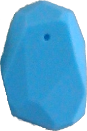
\includegraphics[scale=0.1]{Bilder/Beacon}};
%\node[above left] (P1) at (Beacon1) {$P_1$};
\node[anchor=mid,inner sep=0] (Beacon2) at (0,3){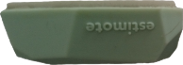
\includegraphics[scale=0.08]{Bilder/BeaconOben}};
\node[anchor=mid,inner sep=0] (Beacon3) at (3,-0.11){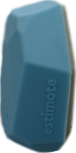
\includegraphics[scale=0.08]{Bilder/BeaconSeite}};
\node[anchor=north east,inner sep=0] (Robo) at (0.4,0.4){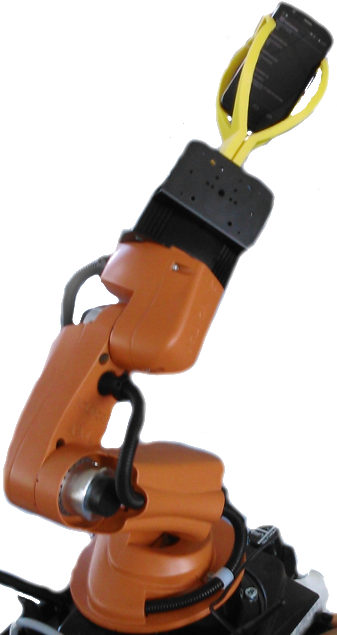
\includegraphics[scale=0.2]{Bilder/DrehungAlle}};
\draw [thick, ->] (0,0) -- node[above] {$z$} ++(Beacon1);
\draw [thick, ->] (0,0) -- node[left] {$y$} ++(Beacon2);
\draw [thick, ->] (0,0) -- node[below] {$x$} ++(Beacon3);
\draw[->] ([shift=(45:3mm)]-0.05,-1.5,0) arc (-40:180:8mm) ;
\end{tikzpicture}
\caption{Skizzierung der Anordnung der Beacons und der Drehung des Roboterarms}
\label{fig:DrehungSkizze}
\end{wrapfigure}
Somit erklärt sich dieses Verhalten nicht anhand der Argumentation, dass eine Antenne bestimmte Charakteristiken aufweist und je nach Winkel der die Qualität des Signals ab- oder zunimmt. Um den Einfluss dieses Phänomens auf die statischen Versuche genauer abzuschätzen, wurden nachfolgend die Messungen aus \ref{sec:MessungBLE} noch einmal wiederholt und lediglich die Drehung um besagte Z-Achse hinzugefügt (siehe Bild \ref{fig:DrehungEinzeln} im Anhang). Die Ergebnisse in der Abbildung verwundert allerdings genauso, denn die fast proportionale Änderung von Ausrichtung zur Stärke der Signalaufnahme ist relativ leicht zu erfassen und sicherlich auch gut zu filtern, doch mit dem Verständnis wie Antennen funktionieren und der bekannten Theorien lässt sich dieses Verhalten nicht erklären. Die einzige Erkenntnis aus den hier durchgeführten Experimenten ist, dass die Vermutung der höchsten Empfangsgüte der Antennen bei normaler Halterung des Smartphones in der flachen Hand sich bewahrheitete und die Richtung, aus denen ein Signal stammt, dabei keinen Einfluss hat.
\begin{figure}[H] 
\centering
\begin{tikzpicture}
\begin{groupplot}[group style={group name=my plots, group size=1 by 4,ylabels at=edge left, vertical sep= 1.5cm}, width=0.7\paperwidth, height=0.15\paperheight, tickpos=left, ytick align=outside, xtick align=outside, enlarge x limits=false]
\nextgroupplot[title={Beacon 1},xticklabels={,,}]
\addplot[color=dblue] table [col sep=comma] {TikzDaten/DrehungAlleBlau.dat};
\nextgroupplot[title={Beacon 2},ylabel={Empfangene Signalstärke in dBm},xticklabels={,,}]
\addplot[color=ice] table [col sep=comma] {TikzDaten/DrehungAlleEis.dat};
\nextgroupplot[title={Beacon 3},xticklabels={,,}]
\addplot[color=mint] table [col sep=comma] {TikzDaten/DrehungAlleMinze.dat};
\nextgroupplot[title={Orientierung in Z-Richtung},xlabel={Zeit in Sekunden},ylabel={Lage in Grad}]
\addplot[solid] table [col sep=comma] {TikzDaten/DrehungAlleAusrichtung.dat};
\end{groupplot}
\end{tikzpicture}
\caption{Verlauf der gemessenen Signalstärke der drei an den Raumachsen befestigten Beacons und der Drehung des Smartphones in Z-Richtung über die Zeit}
\label{fig:DrehungAlle}
\end{figure}
\section{Wechselwirkungen zwischen Funkquellen} 
Unter dem Aspekt der angesprochenen "`Verschmutzung"' eines Raumes durch andere Signalquellen, welche auch im 2,4 GHz Band senden, blieb ein Beweis dieser Behauptungen bisher aus. Der Beweis oder generell die Frage nach Wechselwirkungen mit anderen Transmittern ist insoweit auch wichtig, wenn es um einen Sicherheitsabstand zwischen zwei Beacons geht, bevor sie anfangen sich gegenseitig zu stören. In Bezug auf die generelle Störung von Bluetooth-Signalen durch beispielsweise WLAN-Geräte sind die Auswirkungen weitgehend bekannt und auch hinreichend erforscht (z.B. \cite{InterBLEWLAN}). Jedoch bleibt die Frage, ob sich Beacons untereinander beeinflussen und wenn ja, wie groß der Mindestabstand gewählt werden muss, sodass die Auswirkungen vernachlässigbar sind. Zur Beantwortung wurden die drei verfügbaren Leuchtfeuer relativ nah zueinander befestigt (siehe Abbildung \ref{fig:Dreier}) und zu den gleichen Distanzen, wie in \ref{sec:MessungBLE} die Signalstärken aufgenommen. In Abbildung \ref{fig:DreiZusammen} sind die Ergebnisse aus einem Abstand von 100 cm der Beacons zueinander dargestellt. Im Vergleich zu den Messungen aus \ref{fig:MeterNormal} werden Unterschiede in der empfangenen Signalstärke schnell sichtbar. Das Signal aus dem Beacon-Ansammlung ist bei gleicher Distanz von Beacon zu Smartphone mitunter 5 bis 10 dBm schwächer und deutlich verrauschter (siehe Tabelle \ref{Standardabweichung}), als das Signal von einem alleinstehendem Beacon. Dies beweist somit die grundsätzliche negative Beeinflussung von nah beieinander liegenden Beacons auf deren Sendequalität. In Folge weiterer Untersuchungen ergab sich ein empfohlener Mindestabstand von 50 cm, durch den keine messbaren Verschlechterungen in der Signalstärke mehr vorkamen. An dieser Stelle ist anzumerken, dass hier generell mehr nicht gleich besser bedeutet. Im Hinblick auf die Planung eines Indoor-Lokalisierungs-Systems muss diese Betrachtung in den Gestaltungsprozess mithilfe einer Simulation einfließen, sodass der Sicherheitsabstand gewahrt bleibt.
\begin{figure}[H] 
\centering
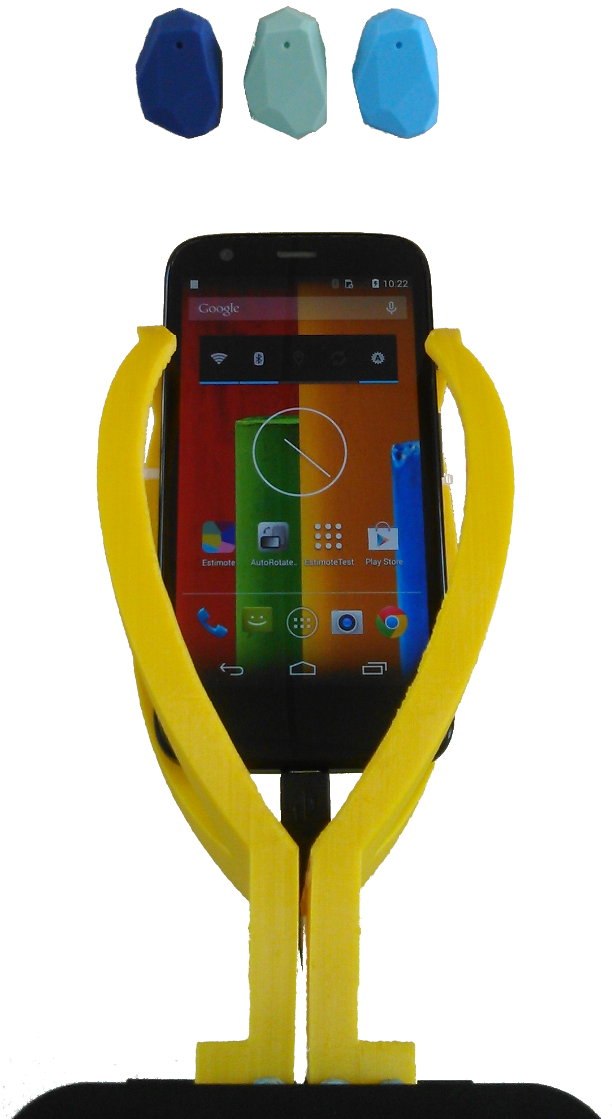
\includegraphics[scale=0.17]{Bilder/MessungBeacon3}
\caption{Gleichzeitige Messung dreier naheliegender Beacon-Signale}
\label{fig:Dreier}
\end{figure}
\begin{figure}[H] 
\centering
\begin{tikzpicture}
\begin{groupplot}[group style={group name=my plots, group size=1 by 3,ylabels at=edge left, vertical sep= 1.5cm}, width=0.7\paperwidth, height=0.15\paperheight, tickpos=left, ytick align=outside, xtick align=outside, enlarge x limits=false]
\nextgroupplot[title={Beacon 1},xticklabels={,,}]
\addplot[color=dblue] table [col sep=comma] {TikzDaten/AlleDreiBlau.dat};
\nextgroupplot[title={Beacon 2},ylabel={Empfangene Signalstärke in dBm},xticklabels={,,}]
\addplot[color=ice] table [col sep=comma] {TikzDaten/AlleDreiEis.dat};
\nextgroupplot[title={Beacon 3},xlabel={Zeit in Sekunden}]
\addplot[color=mint] table [col sep=comma] {TikzDaten/AlleDreiMinze.dat};
\end{groupplot}
\end{tikzpicture}
\caption{Verlauf der gemessenen Signalstärke dreier nah nebeneinander liegender Beacons über die Zeit aus einer Entfernung von einem Meter}
\label{fig:DreiZusammen}
\end{figure}
\begin{table}[H]
\begin{center}
\begin{tabular}{|c|c|c|c|c|}
\cline{3-5}
\multicolumn{2}{c|}{} & \multicolumn{3}{c|}{Standardabweichung} \\
\cline{3-5}
\multicolumn{2}{c|}{} & Beacon 1 & Beacon 2 & Beacon 3 \\
\hline
\multirow{2}{*}{Messung} & aus \ref{fig:MeterNormal} & 0,6946 & 0,8950 & 0,7822 \\
\cline{2-5}
& aus \ref{fig:DreiZusammen} & 0,7316 & 1,6508 & 1,0937 \\
\hline
\end{tabular}
\end{center}
\caption{Standardabweichung der einzelnen Messungen aus \ref{fig:MeterNormal} mit großen Abständen zwischen den Beacons und aus \ref{fig:DreiZusammen} mit geringen Abständen}
\label{Standardabweichung}
\end{table}
\section{Energieverbrauch eines Beacons} 
Der Wartungsaufwand für ein Beacon hängt maßgeblich an der Laufzeit der in jedem Beacon eingebauten Batterie ab. Die in Kapitel 1 und 2 erwähnten Einstellmöglichkeiten von Sendeleistung und der Häufigkeit von Sendeintervallen beeinflussen dabei den Stromverbrauch der Beacons und somit auch die Betriebsdauer der Batterien. Dieser Abschnitt soll sich damit beschäftigen, inwieweit sich die Parameter auf die Wartungszyklen auswirken. Dies soll später dabei helfen, zwischen der Auslegung der beiden Parameter und des gewünschten Wartungsaufwandes abwägen zu können. Denn in großen Projekten mit mehreren hundert Beacons steigt der Wartungsaufwand proportional und wenn einzelne Beacons andere Einstellungen als die Mehrheit aufweisen (um beispielsweise wichtige Gebiete besser abzudecken) wird auch der Überblick über die nötigen Wartungszyklen verloren gehen. Um die Abhängigkeiten zu veranschaulichen, wird anhand vom Datenblatt des verwendeten Hardware-Chips nRF51822\cite{nRF5} in den genutzten Beacons eine Simulation entworfen, die die Einstellmöglichkeiten als Variablen betrachtet. Als Ausgangsbasis für den Energiespeicher wird eine CR2450-Batterie mit 1,8 Wh\cite{CR2450} angenommen. Hierbei wurde nicht vom Idealzustand ausgegangen, sondern ein üblicher Faktor von 0,7 hinzu multipliziert, um der Alterung der Zelle und weiterer Effekte Rechnung zu tragen. Durch die gering fliesenden Ströme und der minimalen Bauweise der Beacons können auch keine direkten Messungen vorgenommen werden. Zudem kann auch nicht verifiziert werden, wie lange ein Sendeauftrag oder ein Zustand vom Prozessor dauert. Um trotzdem ein gutes Simulationsergebnis zu erreichen, muss tiefer in die Funktionsweise der Beacons geschaut werden. Als größte Unbekannte tritt dabei die Sendedauer auf. Bei einer angenommenen Datenrate von 250Kbit/s und bei einer Größe eines Datenpaketes von 38 Bytes \cite{iBPa} (siehe \ref{fig:iBPa}), dauert eine Sendesequenz rund 1 ms. Die benötigte elektrische Leistung für eine vorher definierte Sendeleistung beträgt dabei ein Vielfaches dessen und ist davon stark nichtlinear abhängig. Die dazu nötigen Beziehungen können anhand des Datenblattes des nRF51822 Chips hergeleitet werden. In diesem Fall wurde ein Polynom 4. Grades als Funktion der einstellbaren Sendeleistung aufgestellt, welches annähernd diese Abhängigkeiten beschreibt. Da die Kommunikation bidirektional ist, existiert auch ein Empfangsmodus, der ebenfalls mit 1 ms Empfangsdauer angenommen wird, aber dessen Modus hingegen einen konstanten Stromverbrauch aufweist.
\begin{figure}[H]
\centering
\begin{tikzpicture}
    \node [block, fill=magenta!20, text width=2cm, minimum height=1.5cm] (Header) {\small Header \\(2 Bytes)};
    \node [block, fill=magenta!20, right=0cm of Header, text width=3cm, minimum height=1.5cm] (MAC) {\small MAC Addresse \\(6 Bytes)};
    \node [block, fill=magenta!20, right=0cm of MAC, text width=2cm, minimum height=1.5cm] (Data) {\small Data \\(30 Bytes)};
    \node [block, fill=blue!20, below=1cm of Data, text width=2cm, minimum height=1.5cm] (Major) {\small Major\\ (2 Bytes)};
    \node [block, fill=blue!20, left=0cm of Major, text width=3cm, minimum height=1.5cm] (UUID) {\small Proximity UUID \\(16 Bytes)};
    \node [block, fill=blue!20, left=0cm of UUID, text width=3cm, minimum height=1.5cm] (Prefix) {\small iBeacon Prefix \\(9 Bytes)};
    \node [block, fill=blue!20, right=0cm of Major, text width=2cm, minimum height=1.5cm] (Minor) {\small Minor\\ (2 Bytes)};
    \node [block, fill=blue!20, right=0cm of Minor, text width=2cm, minimum height=1.5cm] (TX) {\small TX Power\\ (1 Bytes)};
    \draw[very thick,->] (Data) -- (Major);
\end{tikzpicture}
\caption{Anteile eines Datenpakets in der Beacon-Kommunikation auf der MAC-Ebene}
\label{fig:iBPa}
\end{figure}
Bei den tatsächlichen Laufzeiten des Sende- und Empfangsmodus muss jedoch ein Unsicherheitsfaktor eingerechnet werden, sodass nicht der berechnete Wert für eine Übertragung genommen wurde, sondern das Zweifache dessen, um ein weniger idealisiertes Bild für die einzelnen Vorgänge zu gestalten. 
\begin{align*}
t_{TX} &= \text{2 ms} \cdot \text{Intervalle [Hz]} \\
t_{RX} &= \text{2 ms} \cdot \text{1 Hz} \\
t_{CPU} &= t_{TX} + t_{RX} \\
t_{IDLE} &= 1-t_{CPU}
\end{align*}
Da für den Sendevorgang noch zusätzlich der Cortex M0 Prozessor aufgeweckt werden muss und dieser das Paket vorbereitet und bis zum Ende der Sendung abwartet, muss hierfür zusätzlich der Energieverbrauch berechnet werden. Da wie erwähnt eine direkte Leistungsmessung an den Beacons durch die gering fließenden Ströme nicht möglich ist, werden aus dem Datenblatt des Prozessors diese rechnerisch ermittelt. Die aktive Phase des Prozessors für alle Operationen vor und nach einer Sendung werden dabei mit 2 ms Sekunden angenommen, welche exakt der Sende- und Empfangsdauer entsprechen. Der Energiebedarf der Recheneinheit wurde im Datenblatt mit 4,1 mA bei einem Takt von 16 MHZ angegeben. So ergibt sich für den Prozessor eine Leistung von 12,3 mW. Zusätzlich wird der Stromverbrauch im IDLE-Modus (untätige Phase des Prozessors) mit 2,6 $\mu$A angegeben. Aus den genannten Gegebenheiten lassen sich nachfolgende Gleichungen erstellen und damit eine Simulation eines Lebenszyklus von einer Batterie näherungsweise bestimmen:
\begin{align*}
E_{Bat} &=& \text{1,8 Wh} \cdot \text{0,7} &=& \text{1,26 Wh}\\
L_{CPU} &=& \text{4,1 mA} \cdot \text{3V} &=& \text{12,3 mW}\\
L_{TX} &=& \text{Polynom 4. Grades (von 4,7 mA }\sim\text{ 11,8 mA)} \cdot \text{3V} &=& \text{14,1 mW} \sim \text{35,4 mW}\\
L_{RX} &=& \text{6,1 mA} \cdot \text{3V} &=& \text{18,3 mW}\\
L_{IDLE} &=& \text{2,6 } \mu\text{A} \cdot \text{3V} &=& \text{7,8 } \mu\text{W}
\end{align*}
ergeben den Zusammenhang
\begin{align*}
t_{Laufzeit} = \frac{E_{Bat}}{L_{CPU}\cdot t_{CPU} + L_{TX}\cdot t_{TX} + L_{RX}\cdot t_{RX} + L_{IDLE}\cdot t_{IDLE}} 
\end{align*}
und dies ergibt folgendes Simulationsergebniss:
\pgfplotsset{
    colormap/jet,
}
\begin{figure}[H]
\centering
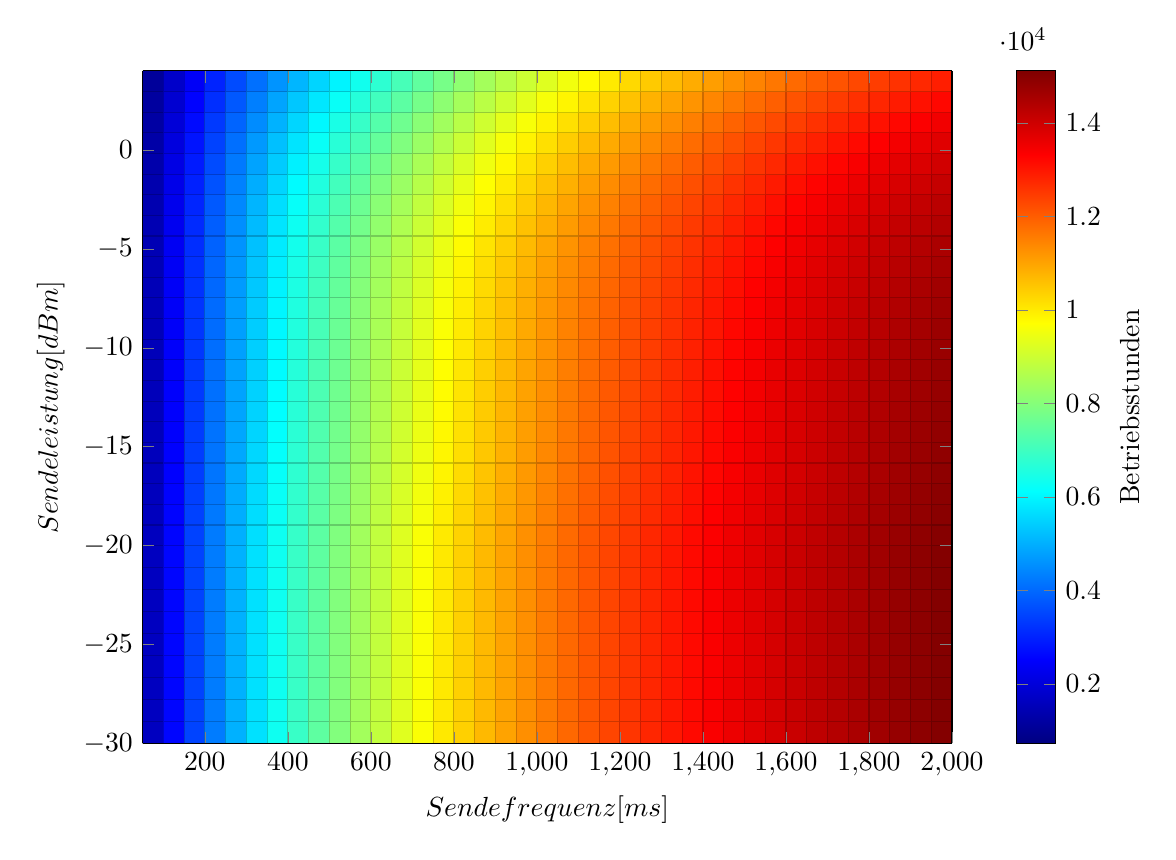
\begin{tikzpicture}
\customrevertcolormap{jet}
\begin{axis}[colorbar, colorbar style={ylabel=Betriebsstunden}, view={0}{90}, xlabel = {$\text{Sendefrequenz [ms]}$}, ylabel = {$\text{Sendeleistung [dBm]}$}, scale=1.5]
\addplot3[surf, samples=40, samples y=10, domain=50:2000, domain y=-30:-20]
{1.8/((4.1e-3 * 3 * 4e-3  * 1000/x) + ((4.2e-5 * (-20) ^ 4 + 2.7e-3 * (-20) ^ 3 + 6.1e-2 * (-20) ^ 2 + 0.65 * (-20) + 8) * 1e-3 * 3 * 2e-3 * 1000/x) + ((6.1e-3 * 2e-3 * 2 + 2.6e-6 * (1 - (4e-3  * 1000/x + 2e-3 * 2))) * 3))};
\addplot3[surf, samples=40, samples y=24, domain=50:2000, domain y=-20:4]
{1.8/((4.1e-3 * 3 * 4e-3  * 1000/x) + ((4.2e-5 * y ^ 4 + 2.7e-3 * y ^ 3 + 6.1e-2 * y ^ 2 + 0.65 * y + 8) * 1e-3 * 3 * 2e-3 * 1000/x) + ((6.1e-3 * 2e-3 * 2 + 2.6e-6 * (1 - (4e-3  * 1000/x + 2e-3 * 2))) * 3))};
\end{axis}
\end{tikzpicture}
\caption{Einfluss der einstellbaren Parameter auf die Lebensdauer einer CR2450-Batterie}
\label{fig:iBBatLe}
\end{figure}
Aufgrund der getroffenen Annahmen würde eine Batterie in den niedrigsten Einstellungen für rund zwei Jahre den Betrieb eines Beacons ermöglichen. Im realen Betrieb hatte sich gezeigt, dass eine Batterie schon nach vier bis fünf Monaten gewechselt werden musste. Während dieser Zeit wurden die Einstellungen nicht geändert und bei einer Intervalllänge von 5 Hz und Sendeleistung von -12 dBm belassen. Beides stimmt mit der Simulation ungefähr überein, was noch kein Beweis für die Gültigkeit der Annahmen bedeutet. Jedoch wird der qualitative Verlauf der wechselseitigen Beziehungen von Einstellparameter und Batterielaufzeit skizziert, der als Orientierung zur Auslegung der Parameter benutzt werden kann.